\section{Time Domain Simulations}

Time domain simulations typically rely on direct simulations of the propogation of an EM signal through a structure and evaluating the response in some manner. In this section we shall primarily discuss the use of direct particle beam simulation, that is the simulation of the beams EM profile via a source signal and then subsequently evaluating the trailing field to acquire the wakefield of the source signal and thus the electromagnetic fields in the structure simulated.

\subsection{Direct Simulation of a Particle Beam}

A large majority of time domain simulation codes (ECHO, MAFIA, CST Particle Studio, GdfidL) use a method that in effect simulates the passage of a particle beam through the structure and evaluates the subsequent electromagnetic fields in the structure by this signal. This is done in the following way:

\begin{enumerate}
\item{A signal representing the source bunch is defined using a given profile, and then passed through the structure from a defined starting displacement and at a given velocity. Additionally a line of integration is defined along which the witness signal will be taken. This in effect defines a source bunch and a witness particle.}
\item{The simulation is run for a given period of time to acquire a significant quantity of the wakefield to correctly analyse the frequency components. It can be seen that for both high-Q resonances and low frequencies this requires a longer wakelength, to encompass the long damping time and correctly resolve the signal frequency, respectively.}
\item{The observed signal is subsequently deconvolved from the source signal to obtain a single particle wakefunction.}
\item{This may then be Fourier transformed (using an FFT algorithm or other numerical methods) to acquire the beam coupling impedance.}
\end{enumerate}

These steps are illustrated for clarity in Fig.~\ref{fig:time_domain_beam} using a simple pillbox cavity as an example, using the time domain code CST Particle Studio.

\begin{figure}
\begin{center}
\subfigure[]{
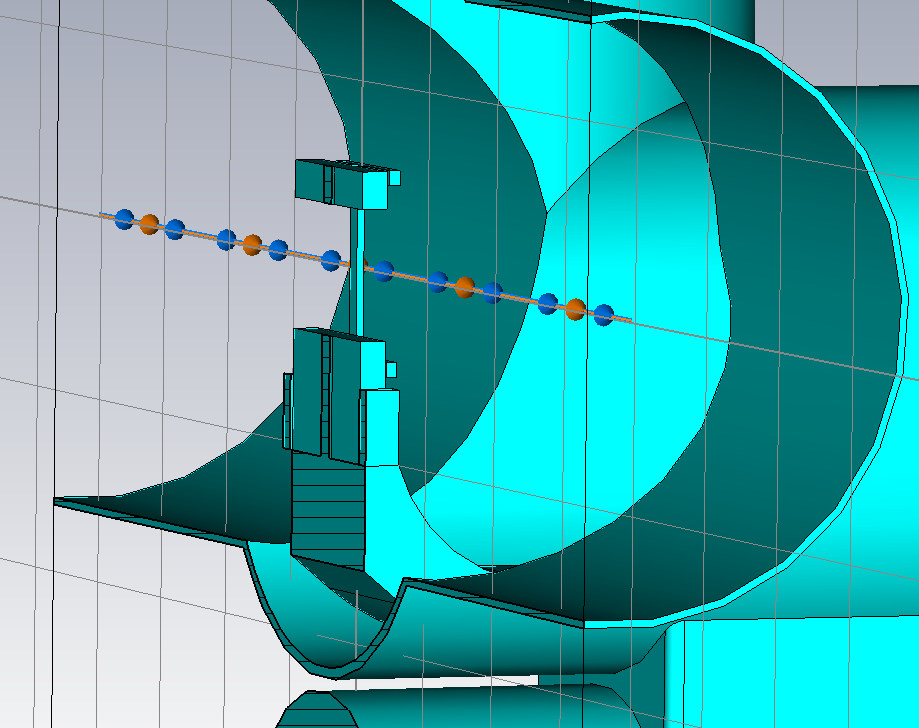
\includegraphics[width=0.45\textwidth]{Computational_Simulations/figures/source-integration-pos.png}
\label{fig:cst_source_signal}
}

\subfigure[]{
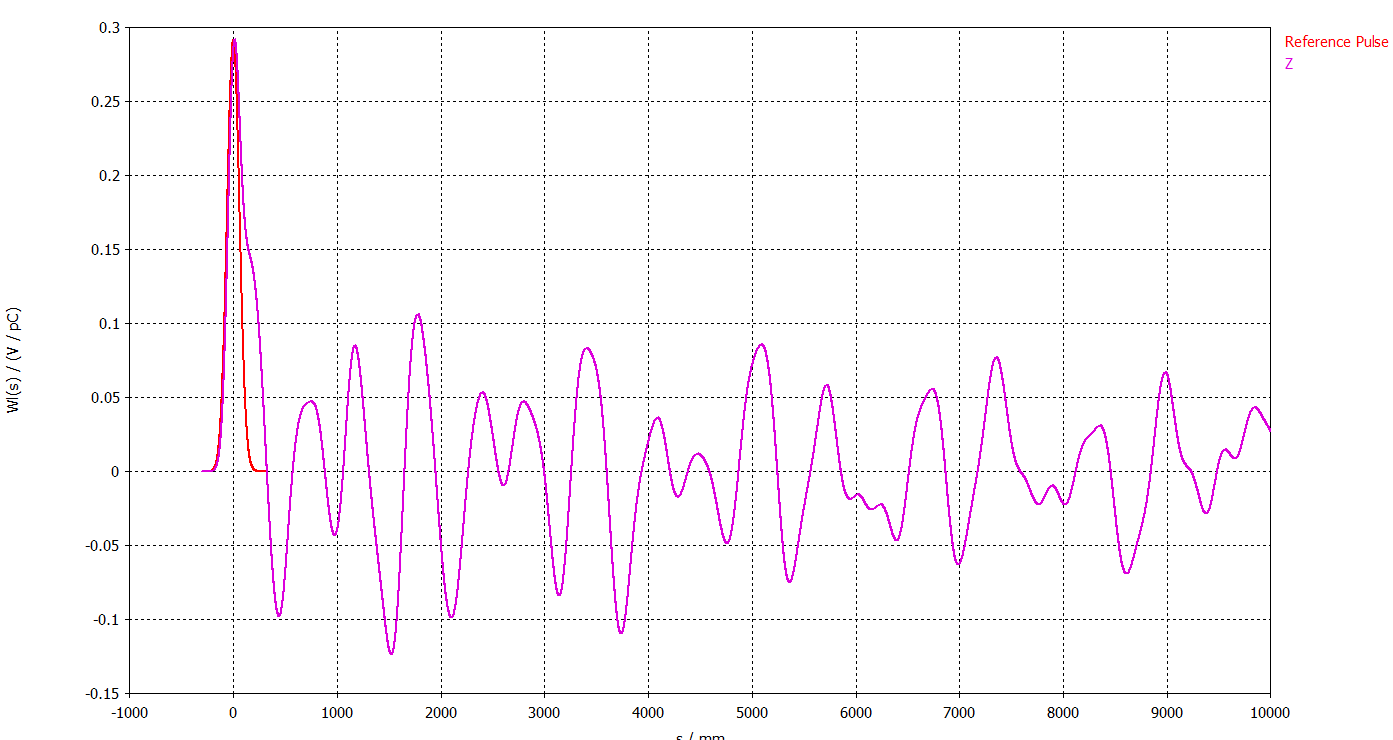
\includegraphics[height=0.5\textwidth]{Computational_Simulations/figures/source-witness-signal.png}
\label{fig:cst_wakepotential}
}
\end{center}
\caption{An illusration of the \subref{fig:cst_source_signal} source signal and witness integration in a time domain code. Here a sample from the UA9 goniometer is shown. The source signal and the resulting wakefield are shown in \subref{fig:cst_wakepotential}.}
\label{fig:time_domain_beam}
\end{figure}

By comparison to the definition of the transverse impedances in Chap.~2, it can readily be seen that by defining either the source signal or witness at different displacements it is possible to acquire both the dipolar and quadrupolar impedances. Additionally, by taking the gradient of the transverse impedances any constant transverse impedance terms can also calculated.
